% C.24 正方形 2, E 为 BC 中点
\documentclass[tikz,border=4pt]{standalone}
\usepackage{ctex}
\usepackage{amsmath}
\usetikzlibrary{calc, arrows.meta}
\begin{document}
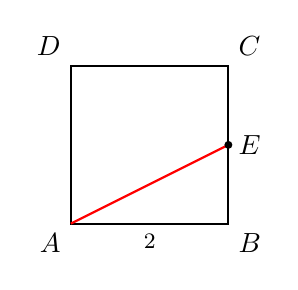
\begin{tikzpicture}[scale=1.0, thick]
  \coordinate (A) at (0,0);
  \coordinate (B) at (2,0);
  \coordinate (C) at (2,2);
  \coordinate (D) at (0,2);
  \coordinate (E) at (2,1);
  \draw (A) -- (B) -- (C) -- (D) -- cycle;
  \draw[red] (A) -- (E);
  \filldraw (E) circle (1pt);
  \node[below left] at (A) {$A$};
  \node[below right] at (B) {$B$};
  \node[above right] at (C) {$C$};
  \node[above left] at (D) {$D$};
  \node[right] at (E) {$E$};
  \node[font=\footnotesize, below] at (1,0) {$2$};
\end{tikzpicture}
\end{document}
